\section{Introduction}
Time series (TS) reasoning models (TSRMs) have emerged as a promising direction for enabling LLMs to understand and reason over temporal data~\cite{timeomni1, thoth2026, patra2026}.
Unlike conventional forecasting, TSRMs produce interpretable reasoning chains that explain \textit{why} a particular conclusion follows from the data.
However, existing TSRMs are primarily developed 
%and evaluated 
on general domains and perform poorly 
%when applied to 
on
financial TS~\cite{merrill2024towards}.
%When we evaluate state-of-the-art TSRMs on financial reasoning tasks in a zero-shot setting, accuracy barely exceeds chance level, confirming that \textit{existing TSRMs lack financial reasoning capabilities}.
%We find that state-of-the-art TSRMs achieve accuracy barely above chance level on financial reasoning tasks in a zero-shot setting, confirming their lack of financial reasoning capabilities.
We find that existing 
%reasoning 
models achieve accuracy barely above chance level on financial reasoning tasks, confirming that \textit{existing TSRMs lack financial reasoning capabilities}.


\textit{\textbf{Why do TSRMs fail on finance?}}
Financial TS exhibit characteristics that fundamentally differ from general domains,
including volatility clustering, momentum and mean-reversion dynamics, support and resistance levels, and complex cross-asset dependencies.
More importantly, financial reasoning involves two distinct modes that existing TSRMs fail to distinguish:
% \setlist[itemize]{leftmargin=0.3cm, itemsep=0.2pt, parsep=0pt, topsep=1pt} for arxiv
\setlist[itemize]{leftmargin=0.56cm, itemsep=1.2pt, parsep=1.2pt, topsep=1pt}
\begin{itemize}
% \item \textbf{Assessment} (\textit{``What is the current state?''}): Deterministic reasoning that can be resolved by computing observable quantities from the price data. For example, measuring drawdown severity or classifying the volatility regime requires only arithmetic on the input prices.
\item \textbf{[1] Assessment} (\textit{``What is the current state?''}): \textit{Deterministic} reasoning that can be resolved by computing observable quantities from price data (e.g., measuring drawdown severity).
% \item \textbf{Prediction} (\textit{``What will happen next?''}): Probabilistic reasoning under uncertainty, where the outcome depends on unobservable external factors such as earnings announcements, macroeconomic shifts, or sector rotation. Even a perfect model cannot achieve 100\% accuracy because the information needed to determine the answer is not fully contained in the price history.
\item \textbf{[2] Prediction} (\textit{``What will happen in the future?''}): \textit{Probabilistic} reasoning under uncertainty, where outcomes depend on unobservable external factors (e.g., earnings announcements or macroeconomic shifts), 
and even a perfect model cannot achieve 100\% accuracy.
\end{itemize}

\begin{figure}[t]
\vspace{-30pt}
\centering
\begin{minipage}[c]{0.43\textwidth}
\centering
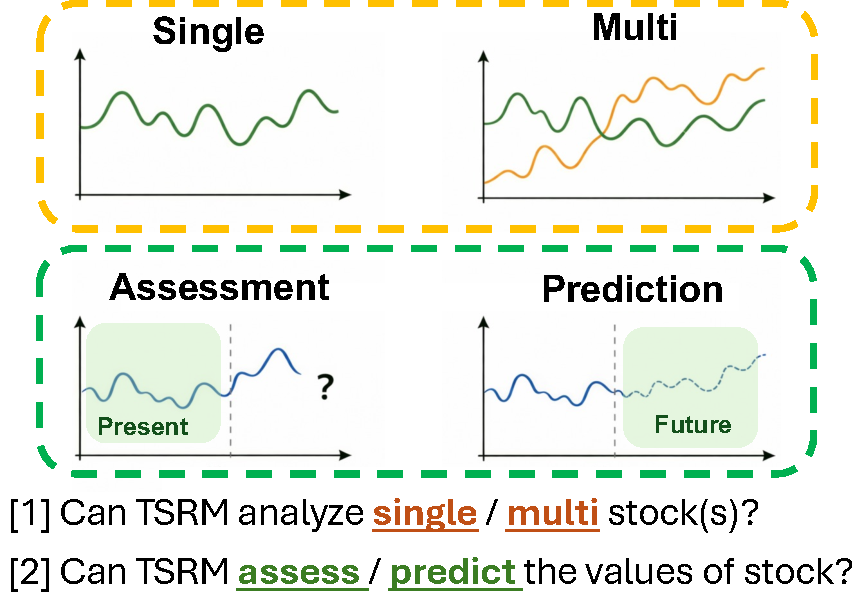
\includegraphics[width=\textwidth]{figures/main.pdf}
\vspace{-12pt}
% \captionof{figure}{Capabilities for Financial TSRM.}
\captionof{figure}{Capability taxonomy for TSRMs.}
\label{fig:taxonomy}
\end{minipage}
\hfill
\begin{minipage}[c]{0.535\textwidth}
\centering
\captionof{table}{
\textbf{Overview of FinTSR-Bench.}
The proposed 
ten financial reasoning tasks
%Tasks 
are organized along two axes: 
% temporal scope (assessment vs.\ prediction) and data scope (single vs.\ multi-stock).
1) \textcolor{darkorange}{\textit{Data}} scope (single-stock vs.\ multi-stock) and 
2) \textcolor{deepgreen}{\textit{Temporal}} scope (assessment vs.\ prediction).
}
\label{tab:taxonomy}
\adjustbox{max width=\textwidth}{
% \small
\begin{tabular}{c|c|c}
\toprule
 & \textcolor{darkorange}{\textbf{Single}} & \textcolor{darkorange}{\textbf{Multi}} \\
\midrule
\multirow{3}{*}{\textcolor{deepgreen}{\textbf{Assessment}}} & Drawdown, & \multirow{3}{*}{Correlation} \\
 & Volatility, & \\
 & Trend & \\
\hline
\multirow{4}{*}{\textcolor{deepgreen}{\textbf{Prediction}}} & Event Response, & \multirow{4}{*}{\shortstack{Relative Performance,\\Pair Convergence}} \\
 & Support/Resistance, & \\
 & Drawdown Recovery, & \\
 & Volatility Forecast & \\
\bottomrule
\end{tabular}
}
\end{minipage}
\vspace{-8pt}
\end{figure}

% \begin{table}[t]
% \vspace{-34pt}
% \centering
% \caption{\textbf{Comparison with related works.} We compare across 1) domain, 2) input modality, 3) task, 4) CoT, and 5) uncertainty modeling. 
% %FinSTaR is the only method that combines all five dimensions for financial TS reasoning.
% FinSTaR is the first TSRM designed for financial TS reasoning.
% }
% \label{tab:comparison}
% \vspace{5pt}
% \adjustbox{max width=\textwidth}{
% \begin{tabular}{l|c|cc|c|c|c}
% \toprule
% \multirow{2.5}{*}{\textbf{Work}} & \multirow{2.5}{*}{\textbf{Domain}} & \multicolumn{2}{c|}{\textbf{Input}} & \multirow{2.5}{*}{\textbf{Task Type}} & \multirow{2.5}{*}{\textbf{CoT}} & \multirow{2.5}{*}{\textbf{Uncertainty}} \\
% \cmidrule(lr){3-4}
% & & TS & Text & & & \\ 
% \midrule
% S2TS-LLM (NeurIPS'25)~\cite{s2tsllm2025} & \multirow{5}{*}{General} & \ding{51} &  & Analysis &  &  \\
% Thoth (arXiv'26)~\cite{thoth2026} &  & \ding{51} &  & Understanding &  &  \\
% PATRA (arXiv'26)~\cite{patra2026} &  & \ding{51} &  & QA & \ding{51} &  \\
% SenTSR-Bench (AISTATS'26)~\cite{sentsr2026} &  & \ding{51} &  & Reasoning & \ding{51} &  \\
% TimeOmni-1 (ICLR'26)~\cite{timeomni1} &  & \ding{51} & \ding{51} & Reasoning QA & \ding{51} &  \\
% \midrule
% FinTSB (arXiv'25)~\cite{liu2025fintsb} & \multirow{4.5}{*}{\textbf{Finance}} & \ding{51} & & Forecasting &  &  \\
% FinBen (NeurIPS'24)~\cite{finben2024} &  & & \ding{51} & NLP tasks &  &  \\
% CausalStock (NeurIPS'24)~\cite{causalstock2024} &  & \ding{51} & \ding{51} & Forecasting &  &  \\
% \cmidrule{1-1} \cmidrule{3-7}
% \textbf{FinSTaR (Ours)} &  & \textbf{\ding{51}} & \textbf{\ding{51}} & \textbf{Reasoning QA} & \textbf{\ding{51}}  & \textbf{\ding{51}} \\
% \bottomrule
% \end{tabular}
% }
% \vspace{-8pt}
% \end{table}
%%%%%%%%%%%%%%%%%%%%%%%%%%%%%%%%%%%%%%%%%%%%%%%%%%%%%%%%%%%%%%%%%%%%%%%%%%%%%%%%%%%%%%%%%%%%%%%%%%%%%%%%%%%%%%%%%%%%%%%%%%%%%%%%%%%%
% \begin{table}[t]
% % \vspace{-34pt}
% \centering
% \caption{\textbf{Comparison with related works.} We compare across 1) domain, 2) input modality, 3) task, 4) CoT, and 5) uncertainty modeling. 
% %FinSTaR is the only method that combines all five dimensions for financial TS reasoning.
% FinSTaR is the first TSRM designed for financial TS reasoning.
% }
% \label{tab:comparison}
% \vspace{5pt}
% \adjustbox{max width=\textwidth}{
% \begin{tabular}{l|c||c|cc|c|c|c}
% \toprule
% \multicolumn{1}{c}{\multirow{2.5}{*}{\textbf{Work}}} & \multirow{2.5}{*}{\textbf{Venue}} & \multirow{2.5}{*}{\textbf{[1] Domain}} & \multicolumn{2}{c|}{\textbf{[2] Input}} & \multirow{2.5}{*}{\textbf{[3] Task}} & \multirow{2.5}{*}{\textbf{[4] CoT}} & \multirow{2.5}{*}{\textbf{[5] Uncertainty}} \\
% \cmidrule(lr){4-5}
% & & & TS & Text & & & \\ 
% \midrule
% S2TS-LLM~\cite{s2tsllm2025} &  NeurIPS'25 & \multirow{5}{*}{General} & \ding{51} &  & Analysis &  &  \\
% Thoth~\cite{thoth2026} & arXiv'26 &  & \ding{51} &  & Understanding &  &  \\
% PATRA~\cite{patra2026}& arXiv'26 &  & \ding{51} &  & QA & \ding{51} &  \\
% SenTSR-Bench~\cite{sentsr2026}& AISTATS'26&  & \ding{51} &  & Reasoning & \ding{51} &  \\
% TimeOmni-1~\cite{timeomni1}& ICLR'26 &  & \ding{51} & \ding{51} & Reasoning QA & \ding{51} &  \\
% \midrule
% FinTSB~\cite{liu2025fintsb} & arXiv'25& \multirow{4.5}{*}{\textbf{Finance}} & \ding{51} & & Forecasting &  &  \\
% FinBen~\cite{finben2024}& NeurIPS'24 &  & & \ding{51} & NLP tasks &  &  \\
% CausalStock~\cite{causalstock2024}& NeurIPS'24 &  & \ding{51} & \ding{51} & Forecasting &  &  \\
% \cmidrule{1-2} \cmidrule{4-8}
% \multicolumn{2}{c||}{\textbf{FinSTaR (Ours)}} &  & \textbf{\ding{51}} & \textbf{\ding{51}} & \textbf{Reasoning QA} & \textbf{\ding{51}}  & \textbf{\ding{51}} \\
% \bottomrule
% \end{tabular}
% }
% \vspace{-8pt}
% \end{table}
%%%%%%%%%%%%%%%%%%%%%%%%%%%%%%%%%%%%%%%%%%%%%%%%%%%%%%%%%%%%%%%%%%%%%%%%%%%%%%%%%%%%%%%%%%%%%%%%%%%%%%%%%%%%%%%%%%%%%%%%%%%%%%%%%%%%
\begin{table}[t]
% \vspace{-34pt}
\centering
\caption{\textbf{Comparison with related works.} We compare across 1) domain, 2) input modality, 3) task, 4) CoT, and 5) uncertainty modeling. 
%FinSTaR is the only method that combines all five dimensions for financial TS reasoning.
FinSTaR is the 
% \textit{first TSRM designed for financial TS reasoning}.
first \first{TSRM} designed for \first{financial} domain.
}
\label{tab:comparison}
\vspace{5pt}
\adjustbox{max width=\textwidth}{
\begin{tabular}{l|c|cc||c|cc|c|c|c}
\toprule
\multicolumn{1}{c|}{\multirow{2.5}{*}{\textbf{Work}}} & \multirow{2.5}{*}{\textbf{Venue}} & \multicolumn{2}{c||}{\textbf{Contribution}} & \multirow{2.5}{*}{\textbf{[1] Domain}} & \multicolumn{2}{c|}{\textbf{[2] Input}} & \multirow{2.5}{*}{\textbf{[3] Task}} & \multirow{2.5}{*}{\textbf{[4] CoT}} & \multirow{2.5}{*}{\textbf{[5] Uncertainty}} \\
\cmidrule(lr){3-4} \cmidrule(lr){6-7}
& & Benchmark & Model & & TS & Text & & & \\
\midrule
\midrule
S2TS-LLM~\cite{s2tsllm2025} & NeurIPS'25 & & \ding{51} & \multirow{5}{*}{General} & \ding{51} &  & Analysis &  &  \\
Thoth~\cite{thoth2026} & arXiv'26 & & \ding{51} &  & \ding{51} &  & Understanding &  &  \\
PATRA~\cite{patra2026} & arXiv'26 & & \ding{51} &  & \ding{51} &  & QA & \ding{51} &  \\
SenTSR-Bench~\cite{sentsr2026} & AISTATS'26 & \ding{51} & \ding{51} &  & \ding{51} &  & Reasoning & \ding{51} &  \\
TimeOmni-1~\cite{timeomni1} & ICLR'26 & \ding{51} & \ding{51} &  & \ding{51} & \ding{51} & Reasoning QA & \ding{51} &  \\
\midrule
FinTSB~\cite{liu2025fintsb} & arXiv'25 & \ding{51} & & \multirow{5.5}{*}{\first{Finance}} & \ding{51} & & Forecasting &  &  \\
FinBen~\cite{finben2024} & NeurIPS'24 & \ding{51} & &  & & \ding{51} & NLP tasks &  &  \\
CausalStock~\cite{causalstock2024} & NeurIPS'24 & & \ding{51} &  & \ding{51} & \ding{51} & Forecasting &  &  \\
FinZero~\cite{wang2025finzero} & arXiv'25 & \ding{51} & \ding{51} &  &  & \ding{51} & Forecasting &  & \ding{51} \\
\cmidrule{1-4} \cmidrule{6-10}
\multicolumn{2}{c|}{\textbf{FinSTaR (Ours)}} & \textbf{\ding{51}} & \textbf{\ding{51}} &  & \textbf{\ding{51}} & \textbf{\ding{51}} & \first{Reasoning QA} & \textbf{\ding{51}}  & \textbf{\ding{51}} \\
\bottomrule
\end{tabular}
}
\vspace{-8pt}
\end{table}

\newlength{\rowheightA}\setlength{\rowheightA}{5.0em}
\newlength{\rowheightB}\setlength{\rowheightB}{4.8em}
\begin{figure}[t]
\vspace{-28pt}
\centering
\footnotesize

% === Example (a): Volatility Regime (Assessment) ===
(\textbf{Single-Assessment}) \textbf{Volatility Regime}: \textit{Classify recent vs.\ overall volatility ratio. GT: (C) High.}
\vspace{1pt}

\noindent
\begin{minipage}[t]{0.20\textwidth}
\vspace{0pt}%
\parbox[c][\rowheightB][c]{\textwidth}{%
\centering
\vspace{4.4pt}
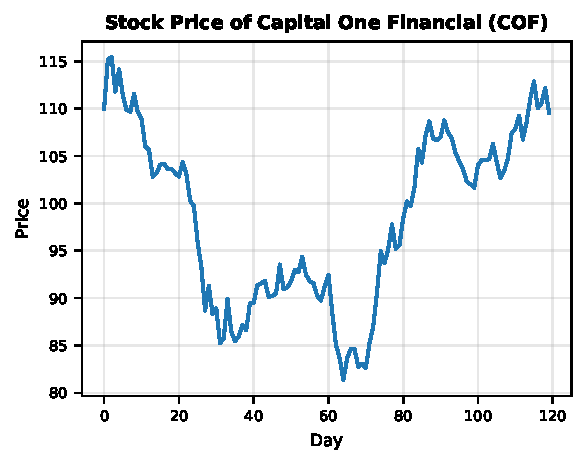
\includegraphics[width=\textwidth]{figures/example_F5_volatility.pdf}}
\end{minipage}
\hfill
\begin{minipage}[t]{0.21\textwidth}
\vspace{0pt}%
\colorbox{red!8}{\parbox[t][\rowheightB]{\dimexpr\textwidth-2\fboxsep}{
\textbf{Qwen2.5-7B} \textcolor{red}{(A)} \ding{55}\\[2pt]
\fontsize{4.5}{5.4}\selectfont
\texttt{Calculate the overall volatility [...] Calculate the recent volatility [...] Compute the ratio [...] Let's perform these calculations.}\\[2pt]
\textcolor{gray}{\textit{$\triangleright$ No computation; directly outputs answer.}}
}}
\end{minipage}
\hfill
\begin{minipage}[t]{0.21\textwidth}
\vspace{0pt}%
\colorbox{red!8}{\parbox[t][\rowheightB]{\dimexpr\textwidth-2\fboxsep}{
\textbf{TimeOmni-1} \textcolor{red}{(B)} \ding{55}\\[2pt]
\fontsize{4.5}{5.4}\selectfont
\texttt{Estimate recent SD $\approx$ 2--3. Estimate overall SD $\approx$ 2--3. Ratio $\approx$ 1.0 $\Rightarrow$ Normal.}\\[2pt]
\textcolor{gray}{\textit{$\triangleright$ Rough estimates; actual recent SD is 10.75\%.}}
}}
\end{minipage}
\hfill
\begin{minipage}[t]{0.35\textwidth}
\vspace{0pt}%
\colorbox{green!10}{\parbox[t][\rowheightB]{\dimexpr\textwidth-2\fboxsep}{
\textbf{FinSTaR (Ours)} \textcolor{green!50!black}{(C)} \ding{51}\\[2pt]
\fontsize{4.5}{5.4}\selectfont
\texttt{Step 1: Compute daily returns.\\
Step 2: Overall volatility = 4.51\%.\\
Step 3: Recent 20-day vol = 10.75\%.\\
Step 4: Ratio = 10.75/4.51 = 2.38.\\
\hspace{0.5em}Recent vol well above long-term avg.\\
$\Rightarrow$ (C) High volatility.}
}}
\end{minipage}

\vspace{10pt}

% === Example (b): Event Response (Prediction) ===
(\textbf{Single-Prediction}) \textbf{Event Response}: \textit{Predict mean-reversion or persistence after a shock. GT: (B) Persistence.}
\vspace{1pt}

\noindent
\begin{minipage}[t]{0.20\textwidth}
\vspace{0pt}%
\parbox[c][\rowheightA][c]{\textwidth}{%
\centering
\vspace{4.4pt}
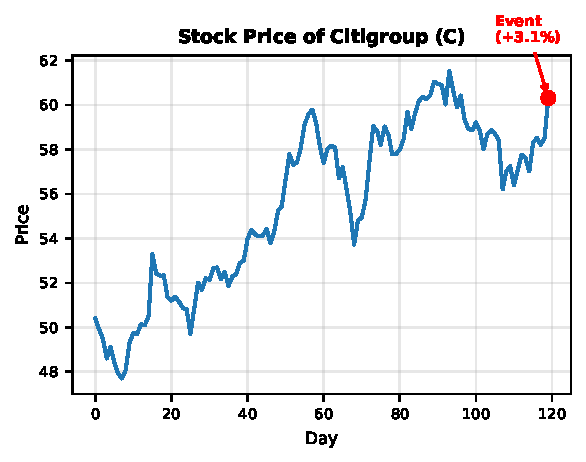
\includegraphics[width=\textwidth]{figures/example_F3_event.pdf}}
\end{minipage}
\hfill
\begin{minipage}[t]{0.21\textwidth}
\vspace{0pt}%
\colorbox{red!8}{\parbox[t][\rowheightA]{\dimexpr\textwidth-2\fboxsep}{
\textbf{Qwen2.5-7B} \textcolor{red}{(A)} \ding{55}\\[2pt]
\fontsize{4.5}{5.4}\selectfont
\texttt{The overall pattern suggests the stock tends to revert to a mean after sharp moves. [...] the most likely outcome is that the price will move back toward pre-event levels.}
}}
\end{minipage}
\hfill
\begin{minipage}[t]{0.21\textwidth}
\vspace{0pt}%
\colorbox{red!8}{\parbox[t][\rowheightA]{\dimexpr\textwidth-2\fboxsep}{
\textbf{TimeOmni-1} \textcolor{red}{(A)} \ding{55}\\[2pt]
\fontsize{4.3}{5.4}\selectfont
\texttt{The last value is 148.40, a significant jump from the previous day's low. This is an outlier [...] mean reversion is the most plausible scenario.}
}}
\end{minipage}
\hfill
\begin{minipage}[t]{0.35\textwidth}
\vspace{0pt}%
\colorbox{green!10}{\parbox[t][\rowheightA]{\dimexpr\textwidth-2\fboxsep}{
\textbf{FinSTaR (Ours)} \textcolor{green!50!black}{(B)} \ding{51}\\[2pt]
\fontsize{4.5}{5.4}\selectfont
\texttt{Step 1: Event: Positive shock, z=4.52, +13.70\%.\\
Step 2: Pre-event trend: downward.\\
Step 3: Scenario analysis:\\
\hspace{0.5em} - Base: Shock reflects genuine new info.\\
\hspace{0.5em} - Adverse: Mean-reversion forces kick in.\\
\hspace{0.5em} - Favorable: Additional news amplifies move.\\
Step 4: 2/3 support Persistence.\\
Step 5: Judgment $\Rightarrow$ (B).}
}}
\end{minipage}

\caption{\textbf{Qualitative comparison.} Two simplified examples where only FinSTaR answers correctly.
Baselines either
fail to compute precise quantities (Volatility Regime)
or
default to heuristic reasoning (Event Response),
while FinSTaR's CoT produces grounded, step-by-step reasoning.
\textcolor{gray}{\textit{Gray italic comments ($\triangleright$) are editorial annotations, not model outputs.}}}
\label{fig:qualitative}
\vspace{-10pt}
\end{figure}


However, no existing TSRM has been specifically designed for the financial domain or distinguishes between these two reasoning modes.
We propose a general $2 \times 2$ capability taxonomy for TSRMs along two orthogonal axes: (data scope) \textit{single-entity vs.\ multi-entity} and (temporal scope) \textit{assessment vs.\ prediction} (Figure~\ref{fig:taxonomy}).
While this taxonomy is applicable to TSRMs in any domain, we instantiate it in the financial domain, where the distinction between deterministic assessment and stochastic prediction is particularly critical,
as ten financial reasoning tasks (Table~\ref{tab:taxonomy}).
To support training and evaluation, we construct \textbf{FinTSR-Bench} from 250 S\&P~500 stocks spanning 2010--2025, with ${\sim}$35K training samples and three out-of-distribution (OOD) test splits for generalization evaluation.

To this end, we propose \textbf{FinSTaR} (\textbf{Fin}ancial Time \textbf{S}eries \textbf{T}hinking \textbf{a}nd \textbf{R}easoning), the first TSRM designed for the financial domain,
as shown in Table~\ref{tab:comparison}.
Trained on FinTSR-Bench, FinSTaR employs different chain-of-thought (CoT) strategies for assessment and prediction.
%Specifically, since assessment is deterministic while prediction is inherently stochastic, \textbf{Compute-in-CoT} for assessment tasks teaches the model to compute answers directly from observable prices, while \textbf{Scenario-Aware CoT} for prediction tasks generates 
Specifically, since assessment is deterministic and prediction is inherently stochastic, we use \textbf{Compute-in-CoT} for assessment tasks to derive answers from observable prices. For prediction, \textbf{Scenario-Aware CoT} generates multiple scenarios before making a probabilistic judgment.
%base, adverse, and favorable 
% various
% scenarios before making a probabilistic judgment.
As illustrated in Figure~\ref{fig:qualitative}, existing models~\cite{qwen2025qwen25,timeomni1} 
either fail to compute precise quantities or rely on heuristic reasoning, 
while FinSTaR's structured CoT produces correct answers through grounded, step-by-step reasoning.
Our main contributions are as follows:
\begin{itemize}
\item We propose a \textbf{general $2 \times 2$ capability taxonomy} for TSRMs by crossing \textit{assessment} vs.\ \textit{prediction} with \textit{single-} vs.\ \textit{multi-entity} analysis, and instantiate it as ten financial reasoning tasks.
\item We construct \textbf{FinTSR-Bench} from 250 S\&P~500 stocks (2010--2025) with 35K training samples
and three OOD test sets for systematic generalization evaluation, each containing 10K samples.
%, 10K samples per test split, and three OOD test sets for systematic generalization evaluation.
\item We propose \textbf{FinSTaR}, trained 
%on FinTSR-Bench 
with different CoT strategies tailored to each reasoning mode: Compute-in-CoT for 
%(deterministic) 
assessment tasks and Scenario-Aware CoT for 
%(stochastic) 
prediction tasks.
\item FinSTaR achieves 78.9\% overall accuracy, outperforming 15+ baselines, including LLMs, TSRMs, and TS forecasting methods. Through systematic ablation, we show that the four capability categories are complementary and mutually reinforcing under joint training.
%, and that Scenario-Aware CoT consistently improves prediction accuracy.
\end{itemize}

